\documentclass[twoside, a4paper, 12pt]{article}
\usepackage{thesis-style}

\usepackage{hyperref}
\usepackage{xcolor}

\usepackage{graphics}
\graphicspath{ {uml/png/} }

\usepackage{amsmath}
%\usepackage{mathbbol}
\usepackage{amsfonts}
\usepackage{amssymb}

% Töltsd ki a saját szakdolgozatod adataival
\def\CIM{Audiovizualiz\'aci\'o val\'os id\H oben\newline\newline Vulkan API-val}
\def\SZERZO{Vida P\'eter}
\def\VEDESEVE{2018}

\def\TANSZEK{Programozási Nyelvek és Fordítóprogramok Tanszék}
\def\TEMAVEZETO{Gera Zolt\'an}
\def\TEMAVEZETOBEOSZTAS{Tan\'arseg\'ed}


\title{\CIM}
\author{\SZERZO}
\date{\VEDESEVE}

\definecolor{light-gray}{gray}{0.95}
\newcommand{\code}[1]{\colorbox{light-gray}{\texttt{#1}}}

\newcommand{\graf}{\mathrm{graf}}
\newcommand{\conj}[1]{\overline{#1}}
%inline fraction
\newcommand{\infrac}[2]{#1/#2}
\newcommand{\vecc}[1]{\mathbf{#1}}
\newcommand{\hz}{\ \mathrm{Hz}}
\newcommand{\scalmul}[2]{\left<#1,#2\right>}

\setcounter{tocdepth}{5}
\setcounter{secnumdepth}{6}

\begin{document}
\pagestyle{empty}

% belső fedőlap
\begin{titlepage}

\begin{minipage}{0.40\linewidth}
\includegraphics[scale=0.3]{img/elte-cimer}
\end{minipage}
\begin{minipage}{0.50\linewidth}
\begin{center}
Eötvös Loránd Tudományegyetem \\
Informatikai Kar \\
\TANSZEK
\end{center}
\end{minipage}

\hrule
\vfill

\begin{center}
\Huge
\textbf{\CIM}
\normalsize
\end{center}

\vfill

\begin{minipage}[t]{0.5\linewidth}
\begin{flushleft}
\textbf{\TEMAVEZETO} \\
\TEMAVEZETOBEOSZTAS
\end{flushleft}
\end{minipage}
\begin{minipage}[t]{0.5\linewidth}
\begin{flushright}
\textbf{\SZERZO} \\
Programtervező Informatikus BSc
\end{flushright}
\end{minipage}

\vfill

\begin{center}
Budapest, \VEDESEVE
\end{center}

\end{titlepage}

\cleardoublepage

% a belső fedőlap utáni lap a témabejelentő

% tartalomjegyzék
\tableofcontents
\cleardoublepage

\pagestyle{plain}
\setcounter{page}{1}

% tartalom
% Ajánlott minden fő fejezetet külön fájlba írni, pl.:

%\tableofcontents


\section{Bevezet\H o}
Inform\'aci\'o minden\"utt jelen van k\"or\"ul\"ott\"unk. A technol\'ogia fejl\H od\'es\'evel egyre t\"obbet \'es t\"obbet tudtunk bel\H ole digitaliz\'alni. Ez\'altal az adat rendelkez\'esre \'all, a k\'erd\'es az marad, hogy ezt hogyan tudjuk felhaszn\'alni.

Az ut\'obbi id\H oben jobban el\H ot\'erbe ker\"ult a vide\'ok\'arty\'ak nem csak j\'at\'ekokban val\'o kihaszn\'al\'asa, hanem nagym\'ert\'ekben t\"obbsz\'alas\'ithat\'o probl\'em\'ak nagy bemenetre val\'o felhaszn\'al\'asa.

Ugyanakkor a nagyobb sz\'am\'it\'asi kapacit\'as nem sokat \'er, ha a programoz\'o nem tudja kihaszn\'alni.
Vide\'ok\'arty\'ak \'altal\'anos c\'el\'u programoz\'asra a mostan\'aban jellemz\H o technol\'ogi\'ak a CUDA az NVIDIA-t\'ol illetve az OpenCL a Khronos Group-t\'ol. A CUDA nagyon gyors \'es el\'eg k\'enyelmes, a sok be\'ep\'itett funkci\'o j\'ovolt\'ab\'ol, amik nem csak levesznek a fejleszt\H o v\'all\'ar\'ol felel\H oss\'eget, de a v\'egletekig optimaliz\'alva van a hardverre. Cser\'ebe csak a gy\'art\'o vide\'ok\'arty\'ain t\'amogatott.
Az OpenCL egy ny\'ilt szabv\'any, \'es nem csak vide\'ok\'arty\'akon val\'o futtat\'ast t\'amogat, hanem egy\'eb hardvereszk\"oz\"oket is. Viszont a szabv\'any implement\'al\'asa a gy\'art\'ok feladata, amit p\'eld\'aul az NVIDIA nem siet el, \'igy a \H o k\'arty\'aikon nem olyan friss verzi\'ot t\'amogatnak. Ez mondjuk \'erthet\H o, hiszen nekik megvan a saj\'at eszk\"oz\"uk.
De ha a grafikus feladatokat n\'ezz\"uk az OpenGL egyre ink\'abb alulmaradt a DirectX-szel szemben, mind haszn\'alhat\'os\'ag, mint teljes\'itm\'eny szempontj\'ab\'ol.

Az OpenGL-\'ert felel\H os \href{https://www.khronos.org/}{Khronos Group} a 2015-\"os \href{http://www.gdconf.com/}{Game Developers Conference}-n bejelentette a Vulkan-t, mint egy alacsonyszint\H u, cross-platform sz\'am\'it\'asi \'es 3D grafika API.
2016 febru\'arj\'aban pedig kij\"ott az els\H o verzi\'o \'es az\'ota is t\"ort\'ennek fejleszt\'esek, illetve lassan, de egyre t\"obben mutatnak ir\'anta \'erdekl\H od\'est, k\"ozt\"uk p\'eld\'aul a nagyszab\'as\'u \href{https://robertsspaceindustries.com/star-citizen}{Star Citizen}.
%\footnote{\url{https://www.gamestar.hu/hir/star-citizen-directx-12-vulkan-api-226130.html}}

\subsection{Vulkan}
\begin{figure}[h]
	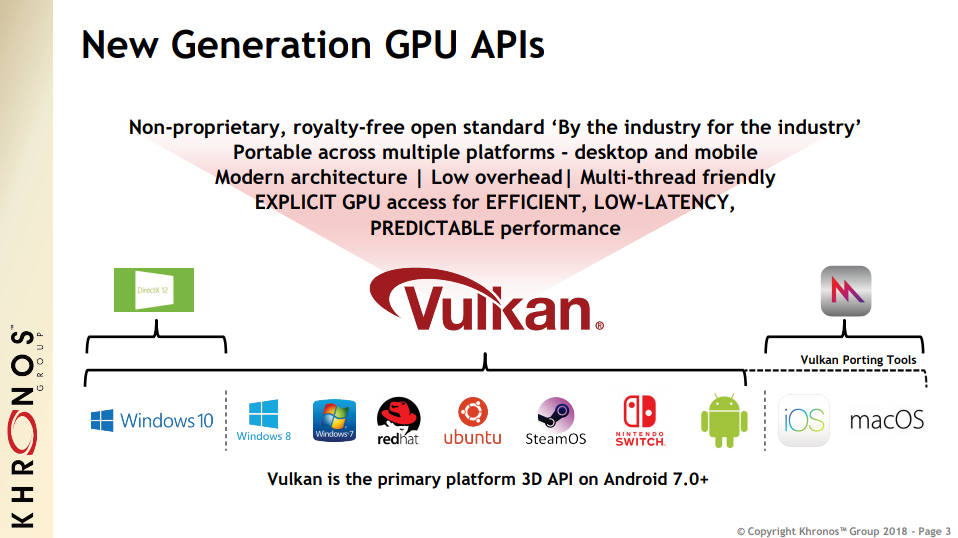
\includegraphics[width=\textwidth]{img/vulkanpromo}
	\centering
	\caption{Prom\'oci\'o az \'uj API-nak.
		\cite{vulkan1.1launchpres} }
\end{figure}
Maga az API az \href{https://www.amd.com/en-us/innovations/software-technologies/mantle}{AMD Mantle} egyfajta folytat\'asak\'ent is tekinthet\H o. Az elgondol\'as az, hogy pr\'ob\'aljunk min\'el jobb teljes\'itm\'enyt kinyerni a hardverb\H ol, CPU-GPU a terhel\'es jobb eloszt\'as\'aval.

A legjobb eredm\'enyhez az vezet, ha optimaliz\'aci\'os lehet\H os\'eget adunk azok kez\'ebe, akik jobban ismerik az adott alkalmaz\'ast: a fejleszt\H ok.
Ez\'altal nagyobb kontrollja van a fejleszt\H onek a program m\H uk\"od\'ese felett, a driverek is egyszer\H ubbek lesznek, ez\'altal a gy\'art\'ok elm\'eletben gyorsabban tudj\'ak az \'uj verzi\'okat t\'amogatni.

Cser\'ebe mivel t\"obb feladatk\"or h\'arul az alkalmaz\'as k\'esz\'it\H o(i)re, maga a fejleszt\'esi folyamat lehet hosszadalmasabb.

\subsection{Kiterjesztett val\'os\'ag}
AR alkalmaz\'asokban a megfelel\H o felhaszn\'al\'oi \'elm\'enyhez elengedhetetlen, hogy kis k\'es\'essel t\"ort\'enjen a felhaszn\'al\'o el\'e az inform\'aci\'o prezent\'al\'asa. 

Kicsit komolyabb p\'eld\'aval \'elve egy j\"ov\H obeli aut\'o AR sz\'elv\'ed\H oj\'en lehet a m\'asodperc t\"ored\'ek\'en m\'ulik egy \'elet, hogy megjelenjen valamilyen figyelmeztet\'es a s\"of\H ornek egy k\"ozelg\H o gyalogosr\'ol.

Tov\'abb\'a a Vulkan \'ig\'erete, hogy a driverek \'ir\'asa egyszer\H ubb lesz, \'igy ebben az esetben lehets\'eges az is, hogy az aut\'o be\'agyazott rendszer\'ere t\"ort\'en\H o fejleszt\'esi id\H o ler\"ovid\"ul, hiszen a fejleszt\H oknek nem kell valamilyen speci\'alisan arra a hardverre fejlesztett k\"ornyezettel megismerkedni\"uk. 

\subsection{Motiv\'aci\'o}



\section{Tervezet}

Az elk\'epzelt jelfeldolgoz\'o rendszer a k\"ovetkez\H ok\'eppen n\'ezne ki. 

\'Altal\'anosan igaz, hogy min\'el magasabb szint\"u egy r\'esz ann\'al k\'enyelmesebb vagy gyorsabb az implement\'aci\'o, ellenben ez a teljes\'itm\'eny rov\'as\'ara mehet. 

\subsection{Jel \'eszlel\'ese} 
Mivel nagyban f\"ugg a hardvert\H ol vagy oper\'aci\'os rendszert\H ol, \'igy el\'eg alacsony szint\H u is \'altal\'aban. 
\'Epp ez\'ert c\'elszer\H unek tartom a feladat\'at minimaliz\'alni.
A digit\'alis jel diszkr\'et volta miatt, meg kell tal\'alni az egyens\'ulyt, hogy mekkora "darabokban" akarjuk \'erz\'ekelni a vil\'agot. P\'eld\'aul mozg\'ast \'erz\'ekelni egy \'all\'ok\'epen neh\'ez, \'es k\"onnyebb lesz min\'el t\"obb k\'ep\"unk van, ellenben ha kis k\'es\'essel szeretn\'enk jelezni a mozg\'ast, nem v\'arhatunk m\'asodperceken kereszt\"ul a sok k\'ep be\'erkez\'es\'eig.

\subsection{Jel \'atalak\'it\'asa}
Miut\'an a jelet \'eszlelt\"uk nyers bitfolyamk\'ent, azt ut\'ana k\"ul\"onb\"oz\H o transzform\'aci\'o(k)nak al\'avetve sz\'amunkra kedvez\H o form\'ara kell hozni. Ez sok mindent jelenthet, a c\'elt\'ol f\"ugg\H oen. Lehet hogy egyszer\H u elemi m\H uveletek, vagy  megfelel\H o tudom\'any\'ag m\'erf\"oldk\"ovei k\"oz\"ott megtal\'alhat\'o bonyolult m\'odszerek, algoritmusok kever\'eke.
Ezekb\H ol tetsz\H oleges mennyis\'eg\H u haszn\'alhat\'o, de \'erdemes a legsz\"uks\'egesebbeket haszn\'alni, \'es r\'eszenk\'ent optimaliz\'alt megold\'ast v\'alasztani. 
C\'elszer\H u lehet tov\'abba min\'el kor\'abban sz\H ur\'est alkalmazni, hogy az esetleges k\"olt\'eges oper\'atorokat min\'el kevesebb adaton kelljen v\'egrehajtani.

\subsection{Visszajelz\'es}
Miut\'an a k\'iv\'ant form\'ara hoztuk az adatainkat, min\'el kisebb overhead-del szeretn\'enk valamilyen visszajelz\'est is kapni fel\H ole. 
Ez egy\'eb ember \'altal \'erz\'ekelhet\H o jelek k\'esz\'it\'es\'et jelenti, \'altal\'aban k\'ep, esetleg hang, vagy ak\'ar haptikus jelz\'esek ad\'asa.
 
\subsection{Hol cs\"okkents\"uk a k\'es\'est?}



\section{Vizsg\'alatok}

A tov\'abbiakban az el\H oz\H o tervezet alapj\'an k\"ul\"onb\"oz\H o k\"onyvt\'arak/API-k felhaszn\'al\'asa \'es \"osszehasonl\'it\'asa a c\'el.


\section{Jelek \'eszlel\'ese}

\subsection{PulseAudio}

\subsection{PortAudio}

\subsection{Jelek feldolgoz\'asa}

A jelfeldolgoz\'asra t\"obb matematikai m\'odszer is van, mind analitikus, mind numerikus t\'eren.
A vizsg\'alat t\'argy\'at most a diszkr\'et Fourier transzform\'aci\'o szolg\'alja.

\subsubsection{FFTW++}
Az \href{http://www.fftw.org/}{FFTW} egy szabad C k\"onyvt\'ar diszkr\'et Fourier transzform\'aci\'o sz\'am\'it\'as\'ara.
E k\"or\'e \'ep\'it kiss\'e bar\'ats\'agosabb \'es k\"onnyebben haszn\'alhat\'o k\"ornyezetet az \href{http://fftwpp.sourceforge.net/}{FFTW++}.
A javaslat az, hogy egy speci\'alis nagyteljes\'itm\'eny\H u \code{Array} oszt\'alyt haszn\'aljunk ezzel.

\"Osszehasonl\'it\'asra ker\"ult az a megold\'as is, ami nem haszn\'alja ezt az oszt\'alyt.

\subsubsection{Sz\'am\'it\'as GPU-n Vulkan-nal}
Ugyanakkor a Vulkan API sz\'am\'it\'asi feladatokat is el tud l\'atni nem csak grafikait. 
Mivel a grafikus visszajelz\'est c\'elszer\H u egy grafikai hardvereszk\"oz seg\'its\'eg\'evel v\'egezni adja mag\'at a lehet\H os\'eg, hogy helyben v\'egezz\"uk a sz\'am\'it\'ast, ezzel kor\'abban elv\'egezve az eszk\"oz saj\'at mem\'ori\'aj\'ara t\"ort\'en\H o m\'asol\'ast.

Mivel egy Vulkan sz\'am\'it\'asi h\'iv\'as aszinkron m\H uk\"odik, a fair \"osszehasonl\'it\'as \'erdek\'eben megv\'arja a m\'er\'es a feladat befejezt\'et. Azonban a p\'arhuzamos\'it\'as miatt, \'es mivel egyazon API haszn\'alat\'ar\'ol van sz\'o, ezt ki lehet haszn\'alni egy\'eb k\'es\H obbi optimaliz\'al\'asokra p\'eld\'aul a megjelen\'it\'es kapcs\'an.

\subsubsection{K\"ornyezet}
A tesztel\H o program megtal\'alhat\'o \href{https://github.com/petii/efop-signalproc}{GitHub-on}. 
A program param\'eterezhet\H o, hogy mekkora alap ablakm\'eret szorz\'okkal futtasson m\'er\'eseket, illetve egyes m\'er\'eseket h\'anyszor ism\'etelje meg. 
Ezeket az adatokat \code{.csv} f\'ajlokba export\'alja. Az adatokat egy egyszer\H u \code{R} szkript seg\'tis\'eg\'evel elemezhetj\"uk.

A teszt bemeneti adatok \href{https://en.cppreference.com/w/cpp/numeric/random/normal_distribution}{pszeudov\'eletlen sz\'amok a standard norm\'alis eloszl\'asb\'ol}.

\subsection{M\'er\'esek}
A k\'et f\H o m\H uvelet ami m\'er\'esre ker\"ult az adatok m\'asol\'asa illetve a DFT futtat\'asa.

\paragraph{Eszk\"oz\"ok}
\begin{itemize}
	\item Egy asztali g\'ep
	\begin{itemize}
		\item \href{https://ark.intel.com/products/80817/Intel-Core-i5-4460-Processor-6M-Cache-up-to-3_40-GHz}
		{Intel Core-i5 4460}
		\item \href{https://www.geforce.com/hardware/desktop-gpus/geforce-gtx-960}
		{NVIDIA GeForce GTX 960}
	\end{itemize}
	\item Egy laptop
	\begin{itemize}
		\item \href{https://ark.intel.com/products/76308/Intel-Core-i5-4300U-Processor-3M-Cache-up-to-2_90-GHz}
		{Intel Core-i5 4300U}
		\item Intel HD Graphics 4400
	\end{itemize}
\end{itemize}

\subsubsection{Eredm\'enyek}



\paragraph{M\'asol\'as}

\begin{figure}[h]
	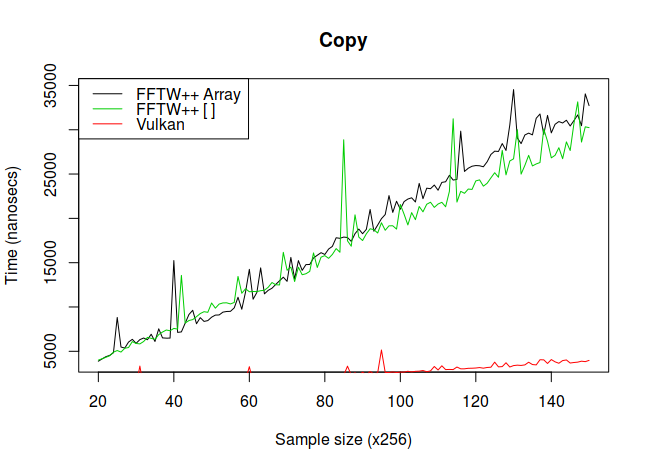
\includegraphics[width=\columnwidth]{copy-l-20-100-150}
	{4300U}
	%\includegraphics[width=\columnwidth]{}
	%{4460}
	\centering
	\caption{M\'asol\'as fut\'asi ideje}
\end{figure}

A m\'er\'esi eredm\'enyeket tartalmaz\'o \'abta $100$ futtat\'as eredm\'enyeinek \'atlag\'at mutatja.

A bemenet \'atm\'asol\'as\'ara ir\'anyul\'o m\'er\'esek olyan szempontb\'ol nem meglep\H oek, hogy nagyj\'ab\'ol line\'aris a bemenet m\'eret\'evel.

\paragraph{Transzform\'aci\'o}

\begin{figure}[h]
	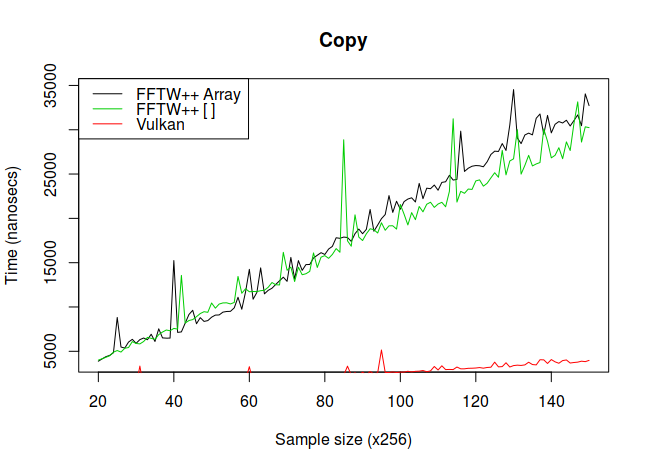
\includegraphics[width=\columnwidth]{copy-l-20-100-150}
	{4300U}
	%\includegraphics[width=\columnwidth]{}
	%{4460}
	\centering
	\caption{Transzform\'aci\'o fut\'asi ideje}
\end{figure}


%
\section{Felhaszn\'al\'oi dokument\'aci\'o}
\subsection{Feladat}
A program azt feladatot hivatott ell\'atni, hogy mikrofonbemenetr\"ol \'erkez\H o hangjelet feldolgozzon, majd ezt az eredm\'enyt vizu\'alisan megjelen\'itse. Mindezt \'ugy, hogy az id\H o ami eltelik a jel \'eszlel\'ese \'es az eredm\'eny megjelen\'ese k\"oz\"ott minim\'alis legyen.
A megjelen\'it\'es egy h\'aromdimenzi\'os spektogramban nyilv\'anul meg. Az $x$-tengelyen az id\H o, az $y$-tengelyen a frekvencia, a $z$-tengelyen pedig az adott frekvenci\'aj\'u hull\'am amplit\'ud\'oja jelenik meg.

\subsection{Technol\'ogia}

\subsection{Hangfeldolgoz\'as}
A jel feldolgoz\'asa vide\'ok\'arty\'an v\'egzett diszkr\'et Fourier-transzform\'aci\'oval t\"ort\'enik. A transzform\'aci\'o a hangjelet az id\H o f\"uggv\'eny\'er\H ol a frekvencia f\"uggv\'eny\'eve alak\'itja. 

\subsection{Rendszerk\"ovetelm\'enyek}\label{runrequirements}
A fejleszt\'es Linuxon, 64 bites AntergOS disztrib\'uci\'on zajlott. Mivel a felhaszn\'alt eszk\"oz\"ok mindegyike cross-platform, \'igy elm\'eletben Windowson is ford\'ithat\'o \'es futtathat\'o a program\footnote{<Vulkan t\'amogatotts\'ag>}, de ez nem ker\"ult tesztel\'esre.

\subsubsection{Vide\'ok\'artya driver}
A haszn\'alt Linux disztrib\'uci\'o csomagjai k\"oz\"ott \'erdemes a \code{vulkan} kulcssz\'ora r\'akeresni \'es a haszn\'alt hardvernek megfelel\"o csomagot/csomagokat feltelep\'iteni.

\subsubsection{???}


\subsection{Futtat\'as}
Ha a futtat\'ashoz sz\"uks\'eges felt\'etelek adottak (\ref{runrequirements}) a program a \code{bin/Release} mapp\'aban tal\'alhat\'o \code{.out} kiterjeszt\'es\H u f\'ajl elind\'it\'as\'aval futtathat\'o. 
%
\section{Fejleszt\H oi dokument\'aci\'o}


\subsection{A feladat r\'eszletes le\'ir\'asa}
\subsubsection{Modell}
Adott egy hangull\'am, ami a leveg\H o nyom\'asa az id\H o f\"uggv\'eny\'eben:
\(s: \mathbb{T} \rightarrow \mathbb{P} \) \newline
A modell\"unkben $\mathbb{T}:=[0,+\infty), \mathbb{P}:=[-1,1] $ \newline
A hanghull\'am, mint \"osszetett rezg\'es fel\'irhat\'o k\"ul\"onb\"oz\H o amplit\'ud\'oj\'u, f\'azis\'u \'es frekvenci\'aj\'u harmonikus rezg\'esek (r\'eszhangok) \"osszegek\'ent, azaz: \newline
\( s(t) = \sum_i r_i\cdot\sin{(f_i\cdot t + \varphi_i)} \), ahol $r_i$ az amplit\'ud\'oja, $f_i$ a frekvenci\'aja, $\varphi_i$ pedig a f\'azisa az $i$-edik r\'eszhangnak.
\subsubsection{Specifik\'aci\'o}
\paragraph{Bemenet}
A modellben szerepl\H o $s$ f\"uggv\'enyb\H ol $\Delta t$ id\H o alatt egy $N$ elem\H u mint\'at v\'etelez\"unk: $s_1,\dots,s_{N}$, \'es \newline
\( \begin{array}{rcl}
s_i := s(x_i) & \text{, ahol } & i\in[1..N],\\
&&x_i\in\{ t_0 = x_0 < x_1 < \dots < x_{N-1} = t_0 + \Delta t \} \text{, tov\'abb\'a } \\
&&x_j - x_{j-1} = \frac{\Delta t}{N}\ (j\in[2..N] ) 
\end{array} \)
\paragraph{Kimenet}
Legyen $\mathbb{F}:=\left[ 0..\frac{N}{2} \right]$\newline>
Ekkor a kimenet egy olyan $R_{s,t_0}:\mathbb{F} \rightarrow [0,+\infty)$ f\"uggv\'eny, amely a frekvencia f\"uggv\'eny\'eben megadja az $s\rvert_{[t_0,t_0+\Delta t]}$ hanghull\'amban az adott frekvenci\'aj\'u r\'eszhang amplit\'ud\'oj\'at, azaz $R_{s,t_0}(f_i) = r_i$.
\paragraph{\'Abr\'azol\'as}
Maga a spektrogram az al\'abbi f\"uggv\'ennyel \'irhat\'o le:
\[ \begin{aligned}[rl]
S&:\mathbb{T}\times\mathbb{F} \rightarrow [0,+\infty), \\
S&(t,f):=R_{s,t}(f)
\end{aligned}
\]
Ekkor az \'abr\'azol\'as az $S$ f\"uggv\'eny grafikonj\'anak, azaz
\[
\graf S = \left\{ \big( (t,f) ,S(t,f) \big) : t\in [0,+\infty), f\in\mathbb{F} \right\}
\]




\subsection{Implement\'aci\'o}

\subsubsection{Architekt\'ura}
Az alkalmaz\'as k\'etr\'eteg\H u modell-n\'ezet architekt\'ura szerint k\'esz\"ult.
Ezek m\H uk\"od\'es\'et a \code{VisaulizationApplication} oszt\'aly k\"oti \"ossze \'es ir\'any\'itja.

\paragraph{Alkalmaz\'as}
\begin{figure}[h]
	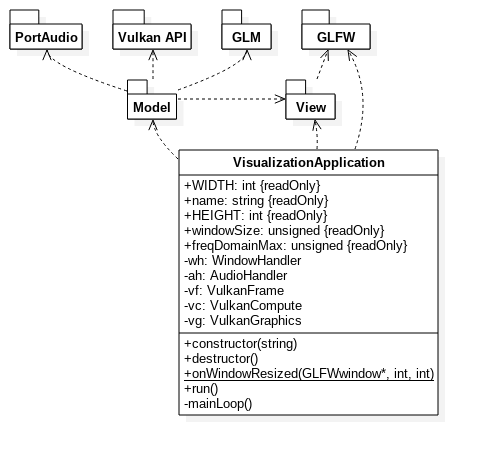
\includegraphics[width=\textwidth]{VisualizationApplication__VisualizationApp_0}
	\centering
	\caption{Az alkalmaz\'as oszt\'alydiagramja \'es a csomagkapcsolatok}
\end{figure}

Az alkalmaz\'as nev\'et a konstruktorban lehet be\'all\'itani, majd a \code{run} met\'odussal elind\'itani. \'Igy a \code{src/main.cpp} f\'ajlban tal\'alhat\'o \code{main} f\"uggv\'enynek csak az alkalmaz\'as futtat\'asa \'es a program sor\'an eldobott kiv\'etelek legv\'egs\H o elkap\'asa lesz a feladata.
Maga az alkalmaz\'as a k\"ovetkez\H o v\'altoz\'okon kereszt\"ul param\'eterezhet\H o:
\begin{itemize}
	\item \code{WIDTH} \'es \code{HEIGHT}: a megjelen\'it\H o ablak kezdeti m\'erete.
	\item \code{windowSize}: mekkora legyen a minta, amit elemz\"unk; a specifik\'aci\'oban $N$
\end{itemize}

\paragraph{N\'ezet}
\begin{figure}[h]
	\includegraphics[width=\textwidth]{View__ViewClassDiagram_2}
	\centering
	\caption{A n\'ezet r\'eteg}
\end{figure}
Az alkalmaz\'as fel\"ulete egy darab megjelen\'it\H o ablakb\'ol \'all, ez a prezent\'aci\'os fel\"ulet.
Ezt a \code{WindowHandler} oszt\'aly biztos\'itja, a GLFW k\"onyvt\'ar seg\'its\'eg\'evel. \newline
A konstruktor\'aban inicializ\'alja a GLFW-t, l\'etrehozza \'es be\'all\'itja az ablakot, be\'all\'itja a hibakezel\H o f\"uggv\'eny\'et. \newline
A \code{getGLFWextensions} f\"uggv\'ennyel inform\'aci\'ot szerezhet\"unk a k\"onyvt\'art\'ol, hogy milyen kieg\'esz\'it\H o funkcionalit\'asokra lesz sz\"uks\'eg\"unk a z\"okken\H omentes m\H uk\"od\'eshez. Ezt felhaszn\'aljuk amikor egy kompatibilis fizikai eszk\"ozt keres\"unk.

\paragraph{Modell}
A modell r\'eteg tov\'abbi r\'eszekre bonthat\'o.
\begin{figure}[h]
	\includegraphics{}
\end{figure}

\subparagraph{Hangkezel\'es}
A hang kezel\'es\'et az \code{AudioHandler} oszt\'aly biztos\'itja.
TODO: interf\'essz\'e alak\'it\'as, \'es k\"ul\"on TestAudioHandler illetve MicAudioHandler.

\subparagraph{Hangfeldolgoz\'as}
A hangfeldolgoz\'as a specifik\'aci\'oban eml\'itett m\'odon diszkr\'et Fourier-transzform\'aci\'oval t\"ort\'enik, ami a \code{VulkanCompute} oszt\'aly seg\'its\'eg\'evel vide\'ok\'arty\'an t\"ort\'enik.
A konstruktor\'aban l\'etrehozza a m\H uk\"od\'es\'ehez sz\"uks\'eges eszk\"oz\"oket. 
\begin{itemize}
	\item A logikai eszk\"ozt, amin kereszt\"ul a program a fizikai eszk\"ozzel kommunik\'alni tud.
	\item A logikai eszk\"ozh\"oz tartoz\'o sort, ahova az utas\'it\'asokat lehet k\"uldeni.
	\item Mem\'ori\'at allok\'al az eszk\"ozon.
	\item Buffereket hoz l\'etre a mem\'oria el\'er\'es\'ere.
	\item L\'etrehozza az er\H oforr\'as le\'ir\'okat.
	\item Bet\"olti a sz\'am\'it\'ast defini\'al\'o shadert.
	\item Sz\'am\'it\'asi cs\H ovezet\'eket hoz l\'etre.
	\item Command pool-t kre\'al \'es command buffer-t foglal bel\H ole.
	\item Felveszi a majd v\'egrehajtand\'o parancsokat a command buffer-be.
\end{itemize}

Ezek ut\'an haszn\'alatra k\'esz, amely sorrendje:
\begin{enumerate}
	\item Adatok felt\"olt\'ese a mem\'ori\'aba a \code{copyDataToGPU} f\"uggv\'eny seg\'its\'eg\'evel.
	\item A sz\'am\'it\'as futtat\'asa a \code{runCommandBuffer} met\'odus megh\'iv\'asa \'altal.
	\item A sz\'amolt eredm\'eny kiolvas\'as\'a a \code{readDataFromGPU} f\"uggv\'ennyel.
\end{enumerate}
TODO: A sz\'amol\'o \'es a rajzol\'o haszn\'aljon k\"oz\"os mem\'ori\'at.

\subparagraph{Rajzol\'as}

%these two may be the same
%\input{tex/dev/application}


\subsection{Fejleszt\'es}
\subsubsection{El\H ok\"ovetelm\'enyek}
\paragraph{Vide\'ok\'artya driver}
L\'asd \ref{gpudriver}.
Amennyiben a Vulkan SDK (\ref{vulkansdk}) telep\'it\'esre ker\"ul, abban megtal\'alhat\'o a bet\"olt\H o r\'eteg.
%A haszn\'alt Linux disztrib\'uci\'o csomagjai k\"oz\"ott \'erdemes a \code{vulkan} kulcssz\'ora r\'akeresni \'es a haszn\'alt hardvernek megfelel\"o csomagot/csomagokat feltelep\'iteni.

\paragraph{GLFW}
A megjelen\'it\H o ablak kezel\'es\'ere a GLFW k\"onyvt\'arat haszn\'alom. Ez szint\'en telep\'ithet\H o csomag a legt\"obb Linux disztrib\'uci\'oban, vagy a \href{http://www.glfw.org/download.html}{weboldalukr\'ol} let\"olthet\H o \'es telep\'it\'esi \'utmutat\'as is megtal\'alhat\'o. 

\paragraph{PortAudio}
Csomagkezel\H o

\paragraph{GLM}
Az OpenGL-b\H ol ismer\H os matematikai k\"onyvt\'ar. 
A telep\'it\'ese t\"ort\'enhet csomagkezel\H on kereszt\"ul, vagy mivel csak fejl\'eceket tartalmaz\'o k\"onyvt\'ar, a megfelel\H o helyre let\"olt\'essel.

\paragraph{Vulkan SDK}\label{vulkansdk}
\subparagraph{Bevezet\H o}
A LunarG Vulkan SDK sz\'amos elengedhetetlen eszk\"ozt tartalmaz. K\"ozt\"uk a sz\"uks\'eges fejl\'eceket, a standard valid\'aci\'os r\'etegeket, debuggol\'o eszk\"oz\"oket \'es a Vulkan f\"uggv\'enyek bet\"olt\H oj\'et.
\subparagraph{Telep\'it\'es}
A haszn\'alt Linux disztrib\'uci\'o csomagjai k\"oz\"ott val\'osz\'in\"uleg megtal\'alhat\'oak fejleszt\'eshez sz\"uks\'eges csomagok. 
\newline
Ellenkez\H o esetben a weboldalr\'ol (\url{https://vulkan.lunarg.com/sdk/home}) let\"olthet\H o a legfrissebb SDK verzi\'o.
A script futtat\'asa ut\'an lesz egy \code{VulkanSDK} mappa az adott k\"onyvt\'arban.
Az ebben tal\'alhat\'o \code{Getting\_Started.html} f\'ajl j\'o kiindul\'opont a tov\'abbiakhoz.
A \code{setup-env.sh} script automatikusan be\'all\'itja a sz\"uks\'eges k\"ornyezeti v\'altoz\'okat.
\subparagraph{Telep\'it\'es tesztel\'ese}
Ezek ut\'an a \code{vulkaninfo}\footnote{A \code{vulkaninfo --html} paranccsal egy k\"onnyeben b\"ong\'eszhet\H o weboldalt kapunk kimenetnek.} parancsot kiadva inform\'aci\'okat kaphatunk a rendszer\"unk k\'epess\'egeir\H ol, illetve tesztelhetj\"uk az SDK telep\'it\'es\'enek sikeress\'eg\'et. 
\'Erdemes lehet tov\'abb\'a p\'eldaprogramokat is lefuttatni. A \code{build\_examples.sh} script leford\'itja a p\'eldaprogramokat, amik ut\'ana a \code{examples/build/} k\"onyvt\'arban megtal\'alhat\'oak. (\code{cube, cubepp})

\subsubsection{Projekt strukt\'ura}
A gy\"ok\'er k\"onyvt\'ar tartalma:
\begin{itemize}
	\item \code{bin}: A leford\'itott futtathat\'o \'allom\'anyok
	\item \code{doc}: Ennek a dokumentumnak a \LaTeX forr\'asf\'ajljai
	\item \code{include}: Az alkalmaz\'as header f\'ajljai (\code{*.h})
	\item \code{src}: Az alkalmaz\'as forr\'asf\'ajljai
	\item \code{test}: Tesztel\'eshez haszn\'alt f\'ajlok
	\item \code{.clang\_complete}: Sz\"ovegszerkeszt\H oh\"oz autocomplete \'es linter plugin configur\'aci\'os f\'ajlja
	\item \code{.git}, \code{.gitignore}: Verzi\'okezel\H o f\'ajljai
	\item \code{README.md}: GitHub-ra "olvass el" f\'ajl
\end{itemize}

\paragraph{\code{bin} k\"onyvt\'ar}
Itt tov\'abbi k\'et alk\"onyvt\'ar tal\'alhat\'o: \code{debug} \'es \code{release). Az el\"obbiben a debug m\'odban ford\'itott alkalmaz\'as, tal\'alhat\'o, amely annyit jelent, hogy gener\'al a \code{gdb} debuggernek plusz inform\'aci\'okat, illetve enged\'elyezi a Vulkan SDK valid\'aci\'os r\'etegeit.
Az ut\'obbiba a release m\'odban ford\'itott alkalmaz\'as ker\"ul. Ez valamivel gyorsabb fut\'ast jelent, cser\'eben az esetleges bugok eset\'en az alkalmaz\'as jobb esetben fut tov\'abb, rosszabb esetben \"osszeomlik, mindenf\'ele inform\'aci\'o a mi\'ertj\'er\H ol mell\H ozve.(\ref{compileoptions})

\paragraph{\code{doc} k\"onyvt\'ar}
A dokument\'aci\'o alapj\'aul az itt tal\'alhat\'o GitHub repository szolg\'alt: \url{https://github.com/shdnx/ELTE-LaTeX-Thesis-Base}

Amiben kieg\'esz\"ult az a projekt:
\begin{itemize}
	\item A \code{szakdolgozat.tex} f\'ajlba \'uj parancsokat vettem fel.
	\item Az \code{uml} k\"onyvt\'arban egy StarUML projekt, a \code{uml/png} k\"onyvt\'arban pedig az UML diagramok tal\'alhat\'oak \code{png} form\'atumban.
	\item A \code{tex} mapp\'aban a tartalmat tov\'abb daraboltam, hogy kisebb, k\"onnyebben \'atl\'athat\'o f\'ajlok rem\'eny\'eben.
		\begin{itemize}
			\item A \code{tex/dev} mapp\'aban tal\'alhat\'oak a fejleszt\H oi dokument\'aci\'o egyes r\'eszei.
		\end{itemize}
\end{itemize}

\paragraph{\code{src} k\"onyvt\'ar}
Ebben a k\"onyvt\'arban tal\'alhat\'oak a ford\'it\'asi egys\'egek.
Tov\'abba itt vannak m\'eg a shaderek is az \code{src/shaders} k\"onyvt\'arban.
A shaderekr\H ol tov\'abbiakat a \ref{shadercompilation} r\'eszben lehet olvasni.

\subsubsection{Ford\'it\'as}
A program gy\"ok\'erk\"onyvt\'ar\'aban a \code{make} parancs kiad\'as\'aval a k\"ovetkez\H ok t\"ort\'ennek:
\begin{enumerate}
	\item Leford\'itjuk a                                                                            shadereket (ld. \ref{shadercompilation})
	\item Leford\'itjuk a programot (ld. \ref{compileoptions})
\end{enumerate}

\paragraph{Ford\'it\'o v\'alaszt\'asa}
A \code{Makefile} elej\'en a \code{COMPILER} v\'altoz\'ot a k\'iv\'ant ford\'it\'ora kell \'all\'itani (\code{g++/clang++}).
\subsubsection{Ford\'it\'asi param\'eterek}\label{compileoptions}
A teljes parancs (a \code{Makefile}-b\'ol): 
\begin{itemize}
	\item Debug verzi\'o
		%\code{\$(COMPILER) -o \$(DTARGET)/\$(OUTPUT_NAME) \$(SOURCES) \$(CFLAGS) \$(INCLUDE) \$(LDFLAGS) -DDEBUG -g -ggdb}
	\item Release verzi\'o
		%\code{\$(COMPILER) -o \$(TARGET)/\$(OUTPUT_NAME) \$(SOURCES) \$(CFLAGS) \$(INCLUDE) \$(LDFLAGS) -DNDEBUG }
\end{itemize}
Itt a k\"ulonb\"oz\H o v\'altoz\'ok:
\begin{itemize}
	\item \code{COMPILER}: A v\'alasztott ford\'it\'o (\code{gcc} vagy \code{clang})
	\item \code{TARGET/DTARGET}: A c\'elmappa (\code{bin/debug} vagy \code{bin/release}) 
	\item \code{OUTPUT\_NAME}: A futtathat\'o \'allom\'any neve
	\item \code{SOURCES}: Az \code{src} k\"onyvt\
	\item \code{CFLAGS}: 
	\item \code{INCLUDE}: 
	\item \code{LDFLAGS}: 
\end{itemize}

\subsubsection{Shader}\label{shadercompilation}
A Vulkan API \href{https://www.khronos.org/spir/}{SPIR-V} shadereket haszn\'al. Mivel ez egy b\'ajtk\'od form\'atum, \'igy a shaderek manu\'alis \'ir\'asa \'es olvas\'asa szokatlan lehet. 
Szerencs\'ere a Khronos Group lefejlesztett egy ford\'it\'ot, ami az OpenGL-b\H ol ismer\H os GLSL shadert SPIR-V shaderr\'e alak\'itja. A LunarG SDK-ban megtal\'alhat\'o ez a program, a 
\code{glslangValidator}. \newline
A GLSL shaderek ford\'it\'asa \'igy t\"obbf\'elek\'eppen is t\"ort\'enhet:
\begin{itemize}
	\item \code{make shaders} \newline
		A \code{Makefile}-ban defini\'alt parancs, leford\'tja az \"osszes shadert a \code{src/shaders} mapp\'aban.
	\item \code{glslangValidator -V src/shaders/<shader neve>.<shader t\'ipusa>} \newline
		A \code{-V} kapcsol\'o mondja meg, hogy gener\'aljon is SPIR-V shadert, an\'elk\"ul csak ellen\H orzi a k\'odot, hogy megfelel-e az implement\'alt szabv\'anynak.
		A shader t\'ipusa alapj\'an az eredm\'enyezett f\'ajl \code{<shader t\'ipusa>.spv} alak\'u. A programba ez alapj\'an a n\'ev lesz bet\"oltve. 
\end{itemize}



\subsection{Tesztel\'es}


\section{\"Osszegz\'es}

\section{K\"osz\"onetny\'ilv\'an\'it\'as}
A projekt az Európai Unió támogatásával, az Európai Szociális Alap
társfinanszírozásával valósul meg (EFOP-3.6.3-VEKOP-16-2017-00002).


\begin{thebibliography}{9}
	\bibitem{citekey}content...
\end{thebibliography}


\end{document}
